% !TEX root = ../../../report.tex
\FloatBarrier
\subsection{Audio Pipelines}\label{subsec:audio_pipelines}

\begin{figure}[H]
    \centering
    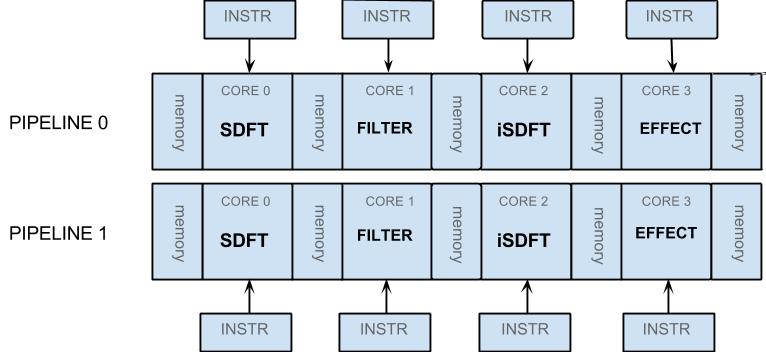
\includegraphics[height=150px]{figures/fpga/system_components_general_pipeline.png}
    \caption{Audio Pipeline Architecture}
    \label{fig:pipeline_architecture}
\end{figure}

\textit{ChaosM} consists of two audio processing pipelines, as illustrated in
Figure \ref{fig:pipeline_architecture}. These contain up to four processing cores
connected by data buffers. Each audio processing pipeline corresponds to one audio channel, operating on audio samples as elementary data elements.
The input/output frequency is directly tied to the sample rate of the input, which acts as a secondary clock input. The main system clock runs on the order of MHz, while this \textit{sample clk} is in the order of kHz and acts as a deadline for when new I/O is due.
